\documentclass{article}
\author{Oliver Kisielius}
\title{Circuit design calculations}
\def\iff{\leftrightarrow}
\def\Z{\mathbb{Z}}
\def\R{\mathbb{R}}
\def\TF{\therefore}
\def\arraystretch{1.3}% Add space between rows of tables.
\usepackage{amsmath}
\usepackage{amssymb}
\usepackage{amsthm}
\usepackage{mathtools}
\usepackage{enumitem}
\usepackage{pdfpages}
\setlength{\parindent}{0pt}
\begin{document}
\maketitle

\section*{Note}

I'm not an electrical engineer. Of course the warning in the MIT license applies to
everything in this repository, but I'll say a few redundant words here.

I've done everything that occurred to me to make the design safe for
people and hardware.  ``Safe for hardware'' means that, if it works
the way I intended, my circuit shouldn't have some failure mode where
the 12 volts from the gaggle of AA batteries ends up ruining the
Raspberry Pi, the load cell, or any other component. But I could be
wrong.

I don't know how I could possibly mess ``safe for people''. But what do I know? I'm not
an electrical engineer.

%% Thanks to this answer:
%% https://stackoverflow.com/questions/2739159/inserting-a-pdf-file-in-latex
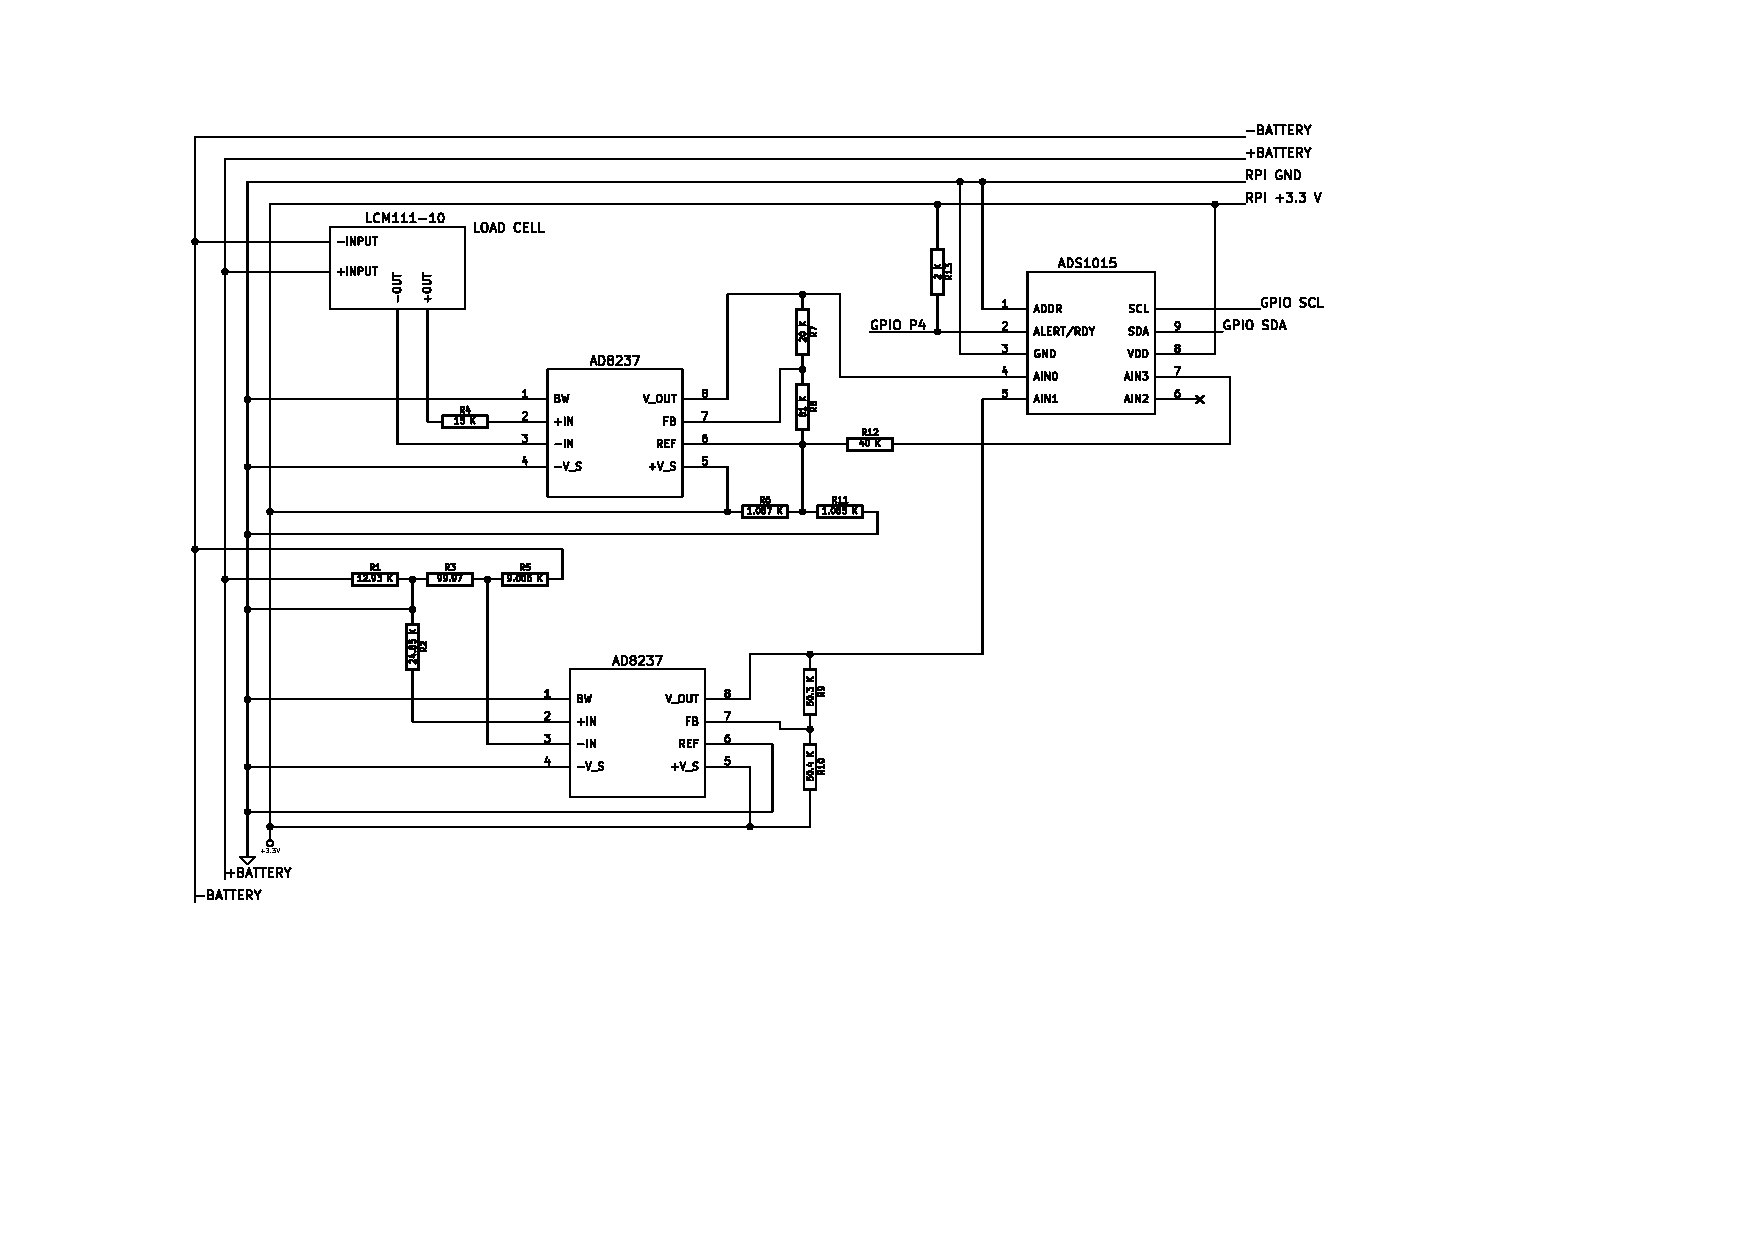
\includepdf[pages={1}]{schematic.pdf}

In broad strokes, here's why I did things the way I did:
\begin{itemize}
\item The AD8237 units are instrumentation amplifiers. You can find their data sheets
  online.
  \begin{itemize}
    \item One AD8237 monitors the battery 

Look at $R_1$, $R_3$, and $R_5$. 

\end{document}
